%****************************************************************%
% FILE: strumentazione.tex                                       %
%****************************************************************%
\documentclass[./main.tex]{subfiles}

\begin{document}
Il percorso di stage ha portato all'acquisizione di nuove conoscenze, non solo teoriche come visto in precedenza per le sorgenti di dati, ma anche pratiche. Questa sezione si occuperà di portare alla luce le conoscenze analizzando gli strumenti utilizzati, sia per lo sviluppo di \textit{Ismar Data} che per la comunicazione tra il team.\par

\paragraph{Comunicazione.}

Quando si entra in una realtà lavorativa è necessario comprendere il modo in cui si affronta il lavoro. In questo caso esso si svolge in modalità mista, che significa che una parte di esso viene fatto online, grazie al cosiddetto \textbf{smart working}.\par

\begin{quote}
\textit{Il lavoro agile o smart working non è una diversa tipologia di rapporto di lavoro, bensì una particolare modalità di esecuzione della prestazione di lavoro subordinato introdotta al fine di incrementare la competitività e di agevolare la conciliazione dei tempi di vita e lavoro\footcite[\url{https://www.lavoro.gov.it/strumenti-e-servizi/smart-working/Pagine/default}]{website-smartworking-ministero-lavoro}.}
\end{quote}

Questo porta alla necessità di stabilire strumenti di comunicazione per consentire il corretto svolgimento del lavoro in team. Le comunicazioni si effettuano utilizzando il software \textbf{slack}\footcite[\url{https://slack.com/intl/it-it/}]{website-slack} che, rispetto all'utilizzo delle classiche mail, consente scambi di messaggi rapidi all'interno di un contesto lavorativo tramite la creazione di appositi canali. Inoltre, come precedentemente accennato, viene usato \textbf{asana} per l'assegnazione e gestione dei compiti seguendo la filosofia \textit{agile}. Ultimo, ma non meno importante, mezzo di comunicazione risulta essere \textbf{google meet}\footcite[\url{https://meet.google.com/}]{website-google-meet}. Una piattaforma di video chiamate fondamentale sia per le review settimanali, dovute all'applicazione del metodo \textit{scrum}, che per qualsiasi delucidazione tra le persone del team.\par

\paragraph{Sviluppo.}
% git
Il codice sorgente del progetto è gestito utilizzando la piattaforma \textbf{GitLab}. Il nome potrebbe far pensare al famoso \textbf{GitHub}, utilizzato da almeno un milione di sviluppatori nel mondo\footcite[\url{https://github.blog/2023-01-25-100-million-developers-and-counting/}]{website-github-100-million-developers}, infatti sono abbastanza simili. Prima di elencare le differenze, occorre dare una panoramica generale su cosa siano le due piattaforme. Innanzitutto entrambe si basano su \textbf{Git}. Git è uno strumento \textit{open source} per il controllo di versione\footnote{Il controllo di versione è un sistema che salva le modifiche fatto a uno o più file nel tempo. In questo modo è possibile richiamare delle versioni specifiche nel tempo futuro. Decisamente più utile rispetto al semplice metodo del copia e incolla in un'altra cartella!} distribuito. In un sistema di controllo di versione distribuito il client\footnote{Con il termine \textit{client} si intende il computer del programmatore.}, oltre ad avere l'ultima versione dei file, ha a disposizione l'intero repository\footnote{\textbf{repository} <ripò$\int$itëri> s. ingl., usato in it. al masch. – Generico ambiente di storage, raggiungibile anche con un percorso web, dove vengono archiviati i pacchetti software che possono essere installati e aggiornati su un computer anche mediante operazioni programmate; \cite{treccani-repository}.}. In questo modo, se il server dovesse avere problemi, ogni persona che ha salvato il progetto in locale\footnote{Con il termine \textit{in locale} si intende il disco fisico nel computer del programmatore.} può poi ripristinarlo nel server\footnote{Con il termine \textit{server} si intende l'elaboratore remoto.}. Git, come illustrato in \autoref{fig:git_snapshot}, pensa ai dati come a una serie di \textit{snapshot} -- \textit{istantanea} -- di un filesystem in miniatura. Fondamentalmente scatta una fotografia di come appaiono i file in quel momento, memorizzandoli solamente in caso il file sia stato modificato, altrimenti memorizza soltanto un collegamento al file già archiviato. Quindi un progetto è visto da Git come un flusso di snapshot.

\begin{figure}[!ht]
\noindent\begin{minipage}{0.5\textwidth}
\vspace{1cm}
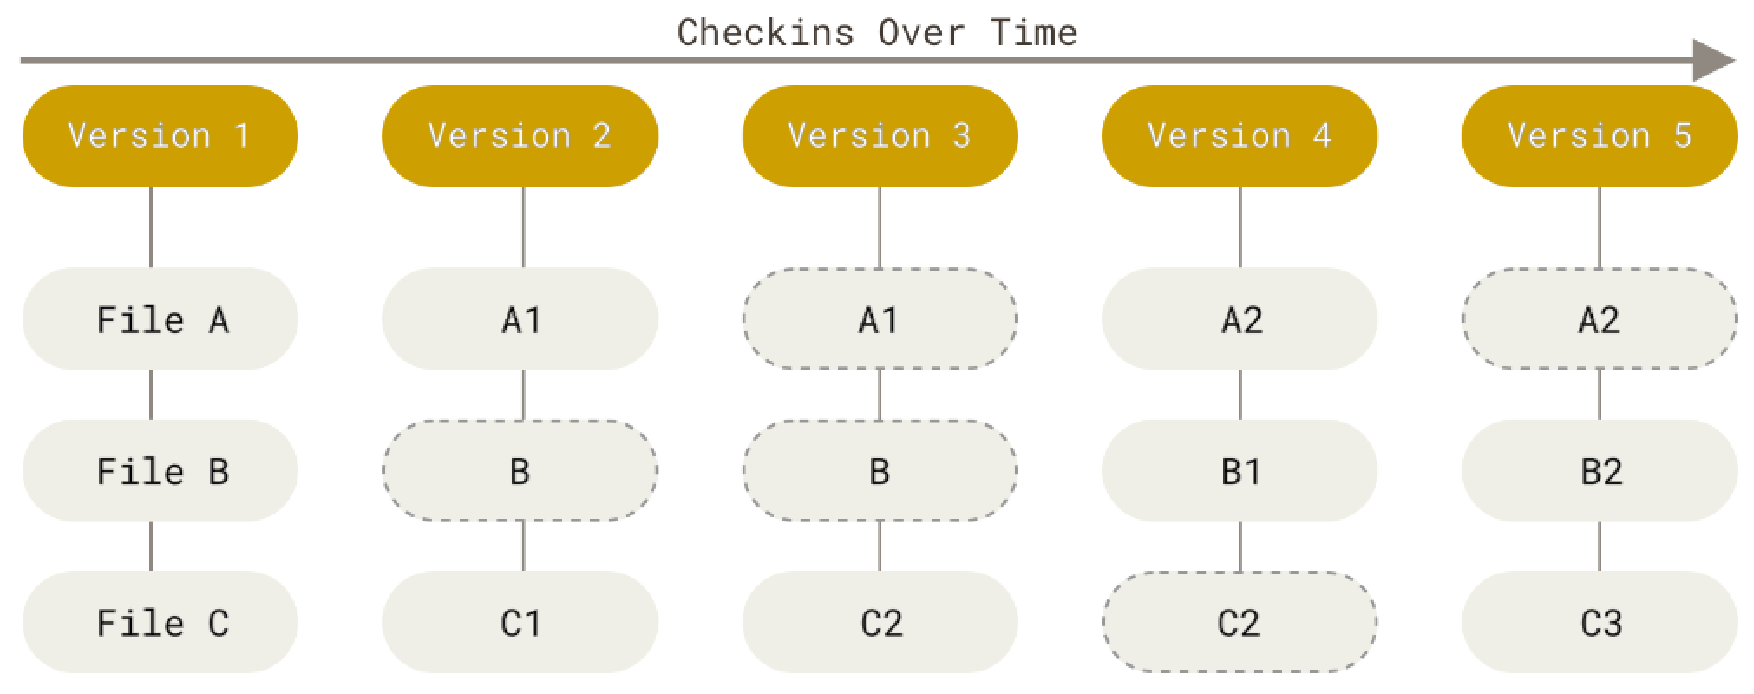
\includegraphics[width=\textwidth]{images/git_snapshot.pdf}
\captionsetup{font=small, hypcap=false}
\captionof{figure}{Flusso di snapshot.}
\label{fig:git_snapshot}
\end{minipage}
\hspace{0.05\textwidth}
\begin{minipage}{0.4\textwidth}
\begin{small}
Immagine rappresentante un esempio di flusso di snapshot effettuato da Git. I blocchi in giallo rappresentano le varie versioni nel tempo, mentre i blocchi in grigio i file del progetto. I contorni tratteggiati indicano un file rimasto invariato nel passaggio di versione.
\end{small}
\end{minipage}
\vspace{0.25cm}
\end{figure}

Un progetto è un insieme di file. Ogni file Git può essere in uno dei seguente tre stati:

\begin{itemize}
    \item \textit{Modified}: il file è stato modificato ma non è ancora stato inserito nel database.
    \item \textit{Staged}: il file viene contrassegnato come modificato nella versione corrente, in modo da poter passare alla successiva.
    \item \textit{Commited}: i dati vengono archiviati al sicuro nel database locale.
\end{itemize}

Ora che i termini principali sono stati chiariti, si può passare alla descrizione di un progetto Git. Esso si compone di tre sezioni (vedi \autoref{fig:git_states}) principali: \textit{working directory}, \textit{staging area}, e \textit{directory Git}.\par

\begin{figure}[!ht]
\noindent\begin{minipage}{0.5\textwidth}
\vspace{1cm}
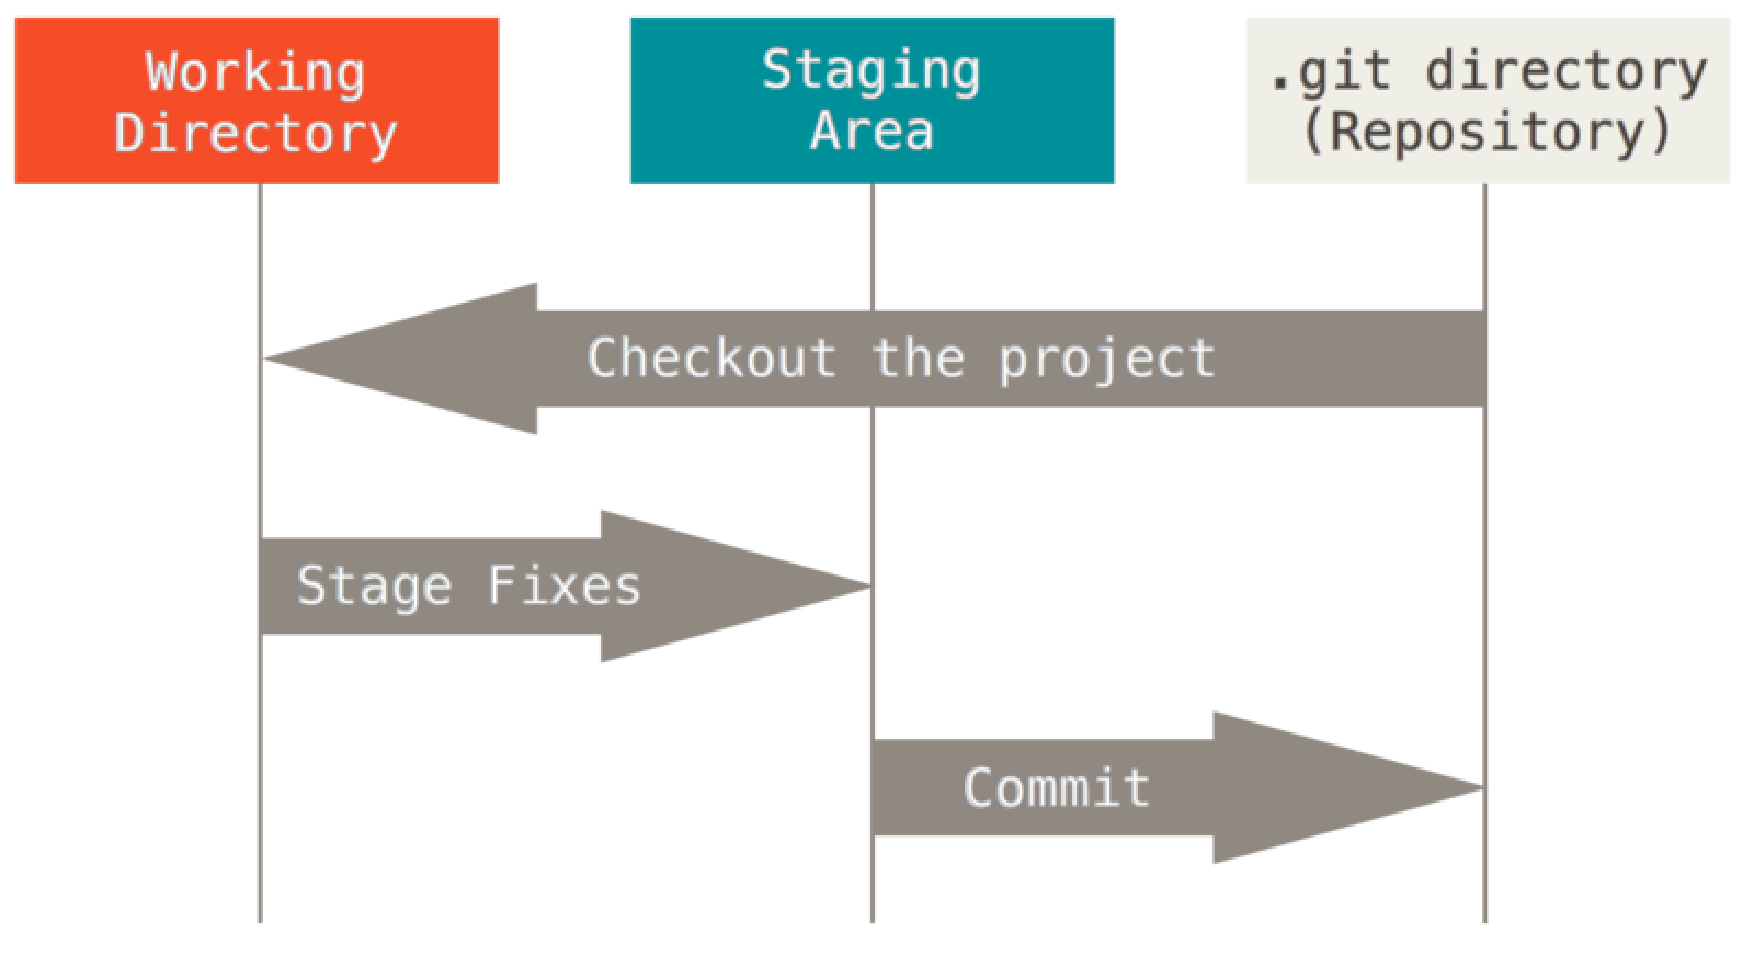
\includegraphics[width=\textwidth]{images/git_states.pdf}
\captionsetup{font=small, hypcap=false}
\captionof{figure}{Working directory, staging area e Git directory.}
\label{fig:git_states}
\end{minipage}
\hspace{0.05\textwidth}
\begin{minipage}{0.4\textwidth}
\begin{small}
Le tre sezioni principali di un progetto Git. Le frecce indicano i passi che devono essere fatti per passare da una parte all'altra.
\end{small}
\end{minipage}
\vspace{0.25cm}
\end{figure}

La working directory -- \textit{cartella di lavoro} --, anche chiamata working tree -- \textit{albero di lavoro} --, rappresenta i file di una singola versione del progetto, estratti dal database di Git e salvati in locale per essere poi modificati. La staging area -- \textit{area di stage} -- è un file nel quale vengono salvate le informazioni per il prossimo commit. Infine la Git directory -- \textit{cartella .git} -- è il cuore del progetto. Dentro la cartella Git salva tutti gli oggetti del database e i meta dati del progetto. Questo è il motivo per il quale essa viene copiata quando si \textit{clona}\footnote{\textbf{clonare} v. tr. [der. di clone] (io clóno, ecc.). \textbf{2. a.} Con uso fig., nel linguaggio dell’informatica, produrre una serie di copie identiche di un elemento di hardware o di software, con partic. riferimento ai calcolatori costruiti come imitazioni di altri di maggiore valore intrinseco e commerciale (ciascuna copia così ottenuta è detta clone); \cite{treccani-clonare}.} un repository. Il flusso di lavoro Git consiste, bene o male, nei seguenti passi:

\begin{enumerate}
    \item Modifica dei file nel \textit{working tree}, mettendoli nello stato \textit{modified}.
    \item Selezionare i file modificati, stato \textit{staged}, per il prossimo commit.
    \item Eseguire i commit, presi dalla \textit{staging area}, memorizzando lo snapshot permanentemente nella \textit{git directory}.\footcite[10-19]{straub-2014}
\end{enumerate}\par

Un ultimo aspetto che occorre evidenziare è il sistema di \textbf{branching}. Come detto in precedenza, Git salva le modifiche come snapshot. A partire dallo snapshot corrente è possibile creare un branch -- \textit{ramo} -- separato. In questo modo, quando sarà effettuato un commit con le modifiche fatte, non andrà ad intaccare il ramo principale. In seguito, tramite l'operazione di \textbf{merge}, è possibile unire il branch separato al principale. Il branch creato di default è chiamato \textit{master}\footcite[63-104]{straub-2014}. Questo sistema permette di avere sempre una versione stabile\footnote{Con il termine \textit{stabile} si intende funzionante e senza che vengano effettuate modifiche direttamente in essa.}.\par

% gitlab
Tornando al discordo principale, GitLab è una piattaforma web che consente di gestire repository Git. Tra le tante funzionalità, non rilevanti per questo testo, c'è la possibilità di creare il proprio repository sui propri server\footcite[\url{https://about.gitlab.com/why-gitlab/\#deployment}]{website-gitlab} (\textit{self-hosted}), questo è il motivo principale per cui nel progetto in questione viene usato esso anziché GitHub. Infatti il repository del progetto per la creazione di \textit{Ismar Data} è ospitato sui server privati di Elan42\footnote{\url{https://repository.elan42.com/progetto-ismar/}}. La \textit{repo}\footnote{\textbf{repo}, abbreviazione informale di repository.} è gestita utilizzando il sistema di branching. In particolare, oltre al master branch, è presente un altro ramo fondamentale, chiamato \textit{develop}\footnote{Quando l'applicazione entrerà in produzione sarà inserito anche un ramo di \textit{staging} contenente la versione del progetto da presentare al cliente.}. Il ramo master contiene la versione finale del progetto, mentre il ramo di develop contiene il codice in corso di sviluppo. Ogni volta che si aggiunge una funzionalità al progetto viene creato (per convenzione interna scelta dagli sviluppatori) un nuovo ramo chiamato \textit{/feature/<nome funzionalità da implementare>}. Durante la review del progetto, se ci sono feature branch completati, se ne effettua il merge in develop in attesa della convalida definitiva da parte del cliente che permetterà di spostare il tutto nel master branch. Un esempio di operazione di merge è mostrata in \autoref{fig:ismarbo_merging}.\par

\begin{figure}[!ht]
\noindent\begin{minipage}{0.5\textwidth}
\vspace{1cm}
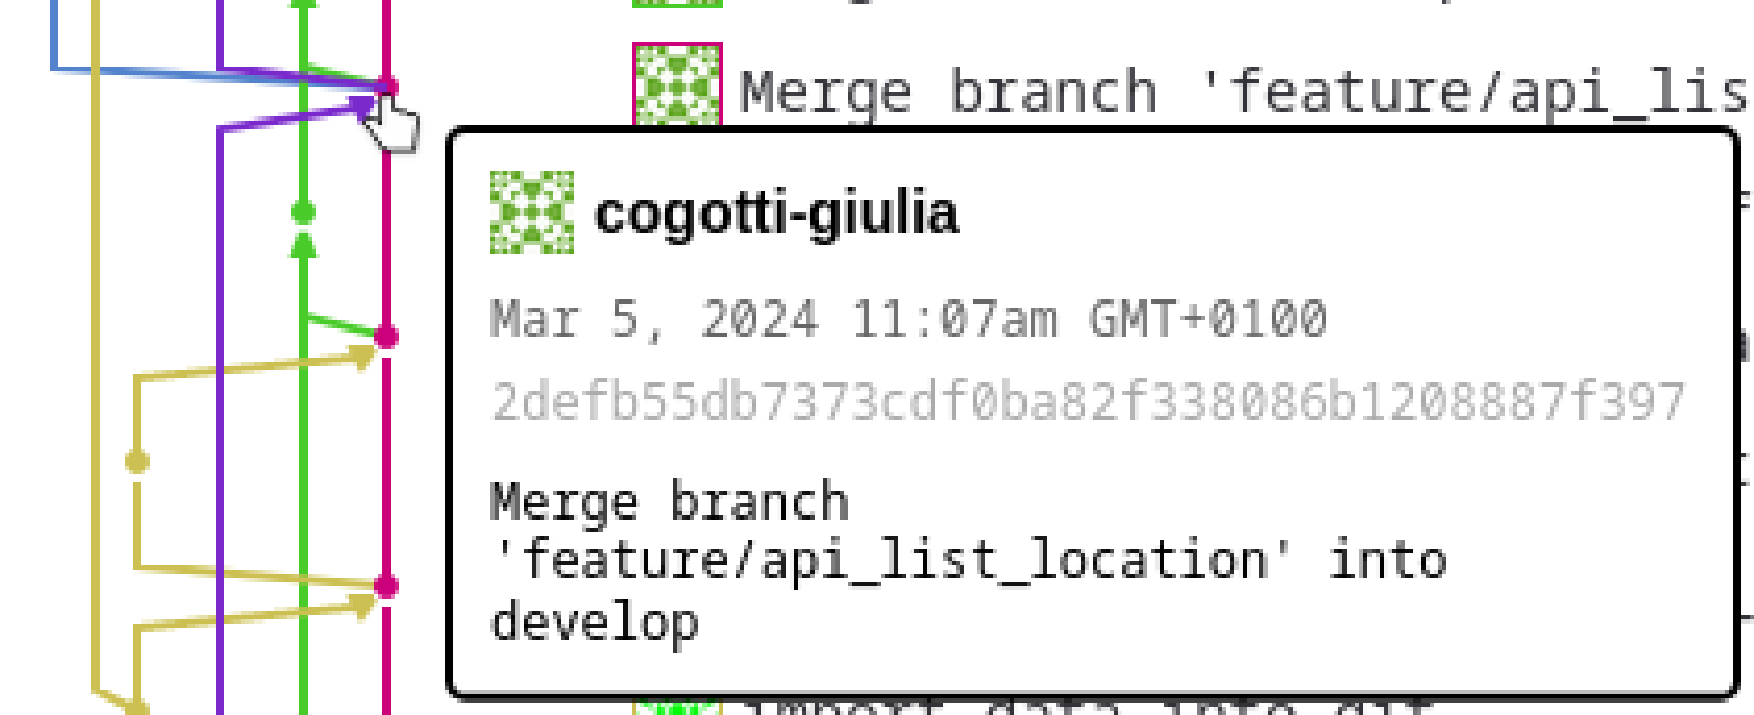
\includegraphics[width=\textwidth]{images/ismarbo_merging.pdf}
\captionsetup{font=small, hypcap=false}
\captionof{figure}{Merge di un feature branch in develop\protect\footnote{Fonte: screenshot dell'autrice.}.}
\label{fig:ismarbo_merging}
\end{minipage}
\hspace{0.05\textwidth}
\begin{minipage}{0.4\textwidth}
\begin{small}
Flusso dei branch in GitLab. In particolare si evidenzia il merging del branch \textit{feature/api\_list\_location} nel ramo di develop.
\end{small}
\end{minipage}
\vspace{0.25cm}
\end{figure}
% vs code
Ogni programmatore clona il progetto in locale e procede ad apportare le modifiche utilizzando l'editor che preferisce, spesso viene utilizzato \textbf{Visual Studio Code} (\textit{VS Code}). Questa risulta essere una delle scelte migliori perché supporta qualsiasi linguaggio di programmazione e, grazie al meccanismo dell'aggiunta di \textit{estensioni}, permette di migliorare la produttività e avere una migliore esperienza utente. Un esempio può essere \textit{Black Formatter}, estensione che permette di formattare il codice scritto in linguaggio Python tramite una semplice combinazione di tasti, senza che il programmatore debba preoccuparsene mentre scrive. Inoltre risulta essere utile quando più programmatori mettono mano allo stesso file, tramite Black si evita di avere un formato visivo diverso che può creare conflitti quando si effettua un commit su Git. Un altro aspetto rilevante è la sua capacità di gestire i flussi di Git, sia a livello di riga di comando che a livello grafico. Infine VS Code è completamente gratuito e funziona su tutti i sistemi operativi di maggior utilizzo\footcite{website-vscode}.\par

\paragraph{Tecnologie.}
%python
Il progetto è sviluppato utilizzando il linguaggio di programmazione ad alto livello \textbf{python}. Python funziona su tutti i principali sistemi operativi (in particolare Linux, Unix, MAC OS X e Windows)\footcite[\url{https://wiki.python.org/moin/BeginnersGuide/Overview}]{website-wiki-python}. Pyhton fornisce una \textbf{libreria standard} -- \textit{standard library } -- contenente moduli integrati (scritti in C) che forniscono accesso a funzionalità di sistema come I/O di file e altri moduli (scritti in Pyhton) che implementano soluzioni per molti problemi che si verificano nella programmazione quotidiana, evitando che il programmatore debba implementarsi tutto da solo e permettendo quindi che si concentri sulle finalità del suo lavoro. Oltre alla standard library, è presente una raccolta di librerie create da vari sviluppatori e distribuite nella repository PyPI\footcite[\url{https://pypi.org/}]{website-pypi}. L'applicazione visualizza dati che seguono alcuni formati standard. È possibile utilizzare alcune librerie di pyhton che aiutano nella conversione dai formati grezzi a ciò che l'utente visualizzerà.\par

% django
L'applicazione, lato back-end, si basa sul framework web \textbf{Django}. Django è gratis ed è open-source. Esso offre un aiuto agli sviluppatori per implementare applicazioni nel modo più veloce possibile. Django applica lo schema chiamato \textit{Model-View-Controller (MVC)}. L'MVC è un modo di sviluppare software in modo che divide il progetto in diversi "livelli". Il codice per la definizione e accesso ai dati (M=model) viene separato dalla logica di instradamento delle richieste (C=controller), che a sua volta è separata dall'interfaccia utente (V=vista). Questo consente la modifica di una parte dell'applicazione in modo indipendente dalle altre parti\footcite[5-10]{the-django-book}. In realtà, dato che la logica di instradamento delle richieste è gestita dal framework stesso, più che MCV risulta essere catalogato come \textit{framework MTV}. In questo modello sono presenti tre livelli principali. Il primo si occupa dell'accesso ai dati (M=model), il secondo della presentazione di essi all'utente, quindi cosa e come visualizzarli (T=template), l'ultimo livello riguarda la logica di accesso ai modelli e come riferirsi al giusto template (V=view)\footcite[62-63]{the-django-book}.\par

% graphql
Il linguaggio utilizzato per prendere i dati dal back-end e passarli al front-end è \textbf{GraphQL}. GraphQL è quindi un linguaggio di interrogazione -- \textit{query} -- per API. Tipicamente, le API in formato REST per prendere e passare i dati necessitano di fare molte chiamate, le API GraphQL invece effettuano una singola chiamata per dare all'applicazione tutto ciò di cui ha bisogno. Questo incrementa la velocità dell'applicazione anche se il dispositivo mobile ha una connessione ad internet lenta. Inoltre, le query GraphQL inviano solamente ciò che viene richiesto dall'applicazione. Questa funzionalità è sicuramente un vantaggio perché il client sa cosa ha richiesto e cosa ottiene, rendendo l'applicazione veloce e stabile. Ma non è finita qui! Considerando i diversi tipi di dati che devono essere passati, sarebbe veramente svantaggioso utilizzare un formato che struttura i dati tutti allo stesso modo. GraphQL fornisce invece adattabilità al contesto\footcite[\url{https://graphql.org/}]{website-graphql}. L'interfaccia grafica \textbf{GraphiQL} consente di utilizzare un ambiente GraphQL direttamente su browser\footcite[\url{https://github.com/graphql/graphiql?tab=readme-ov-file\#graphiql}]{website-graphiql}. La libreria \lstinline{graphene} fornisce strumenti per implementare le API GraphQL direttamente in linguaggio python, senza dover scrivere utilizzando il linguaggio offerto da GraphQL\footcite[\url{https://docs.graphene-python.org/en/latest/quickstart/}]{website-graphene-docs}. Grazie alla libreria python \lstinline{graphene-django} è possibile includere GraphQL nel progetto, con anche l'interfaccia grafica a disposizione (vedi \autoref{lst:graphiql_installedapps}). La libreria in questione è costruita sopra la semplice \lstinline{graphene} e fornisce astrazioni che semplificano l'aggiunta delle funzionalità GraphQL al progetto Django. Quindi nel progetto sarà quest'ultima ad essere utilizzata (vedi \autoref{lst:graphiql_installedapps})\footcite[\url{https://docs.graphene-python.org/projects/django/en/latest/}]{website-graphene-docs}.\par

\begin{lstlisting}[language=Python, caption=settings.py, label=lst:graphiql_installedapps]
INSTALLED_APPS =[
    ...
    "django.contrib.staticfiles", # Required for GraphiQL
    "graphene_django",
    ...
]
\end{lstlisting}

Specificando l'indirizzo a cui accedere (vedi \autoref{lst:graphiql_url}) si ottiene l'interfaccia grafica di GraphiQL in \autoref{fig:grahiql_gui}, che rispecchierà i modelli e le query specificate nel codice python.\par

\begin{lstlisting}[language=Python, caption=urls.py, label=lst:graphiql_url]
from graphene_django.views import GraphQLView
from django.views.decorators.csrf import csrf_exempt

urlpatterns = [
    path("graphql/", csrf_exempt(GraphQLView.as_view(graphiql=True))),
    ...
]
\end{lstlisting}

\begin{figure}[!ht]
\noindent\begin{minipage}{\textwidth}
\vspace{1cm}
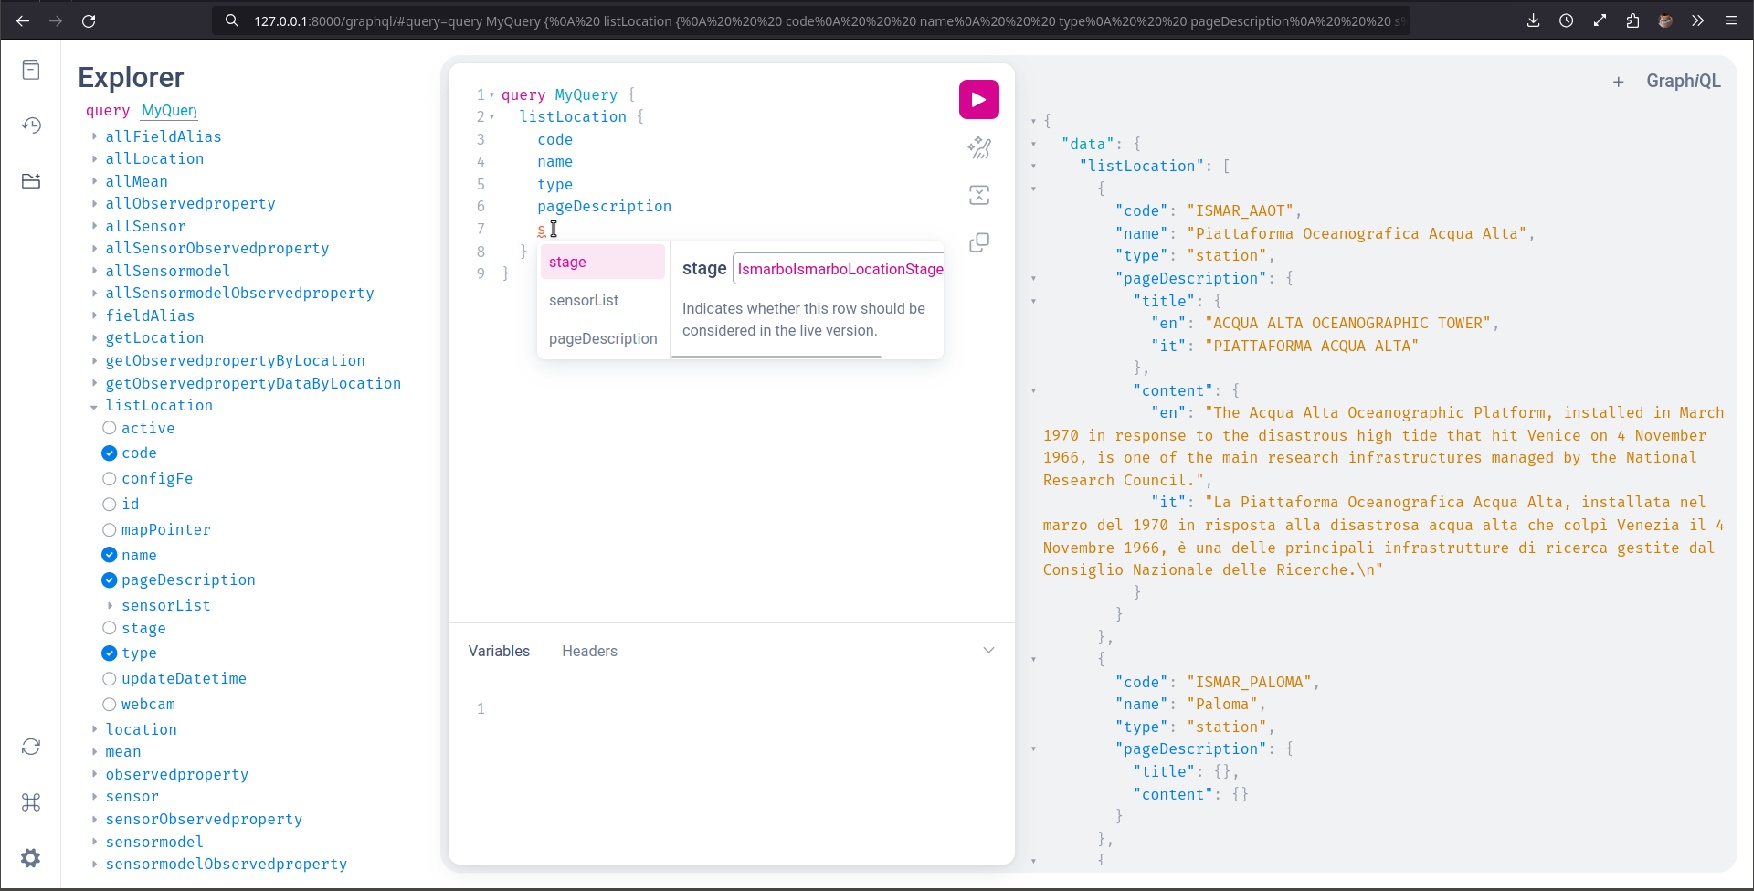
\includegraphics[width=\textwidth]{images/graphiql_interface.pdf}
\captionsetup{font=footnotesize, hypcap=false}
\captionof{figure}{Interfaccia grafica GraphiQL. Al centro l'editor per le query, a destra il risultato dell'esecuzione della query e a sinistra la lista delle query costruite in python e integrate con la libreria \lstinline{graphene-django}\protect\footnote{Fonte: screenshot dell'autrice.}.}
\label{fig:grahiql_gui}
\end{minipage}
\vspace{0.25cm}
\end{figure}

% postgresql
L'applicazione, lato back-end, dispone di un database \textbf{postgreSQL}. Esso segue il \textit{modello relazionale}. È importante evidenziare che esso non sarà decritto con precisione, ne verrà data solo un'idea per chiarire alcuni termini che saranno utilizzati nei successivi capitoli. Lo schema è costituito da \textit{entità} (tabelle) e \textit{relazioni}. Ogni tabella contiene record (detti anche righe o n-uple) differenti. Ogni riga è formata da un certo numero di elementi. Questo numero deve essere uguale per tutti i record della tabella. Ogni n-upla deve essere distinta dalle altre, almeno per un campo, chiamato \textit{chiave}. Esistono tre operatori principali: \textit{selezione} per l'estrazione dei dati, \textit{proiezione} per la scelta di certi campi e \textit{giunzione}. Quest'ultimo è fondamentale per l'unione di due tabelle data la chiave in comune.\footcite[28-40]{doretti-concetti-base-db}.\par

\textbf{SQL}\footnote{Inizialmente acronimo di \textit{Structured Query Language}, ma ormai considerato come un nome proprio. Vi sono due pronunce analoghe anglosassoni: "es-que-el" (in italiano "esse-qu-elle") e, come se fosse una parola intera, "sequel".} è un linguaggio per database relazionali. SQL fornisce sia funzionalità DML (\textit{Data Manipulation Language}), ovvero modifica e interrogazione ad un database, che di DDL (\textit{Data Definition Language}), che consiste in comandi per definire lo schema di un database relazionale. Le tabelle rispecchiano il contenuto di quelle del modello, quindi gli elementi sono gli stessi. In particolare le colonne della tabella vengono chiamati attributi. Qui il concetto di chiave assume molta importanza. È obbligatorio specificare una \textit{chiave primaria} --\textit{primary key (PK)} -- che identifica univocamente una riga della tabella. Ultimo aspetto da evidenziare è il vincolo di \textit{chiave esterna} -- \textit{foreign key (FK)} -- che crea un legame tra i valori di un attributo della tabella su cui è definito e i valori di un attributo in un'altra tabella che è la chiave primaria di tale tabella. In realtà potrebbe accadere anche che i due attributi si trovano nella tabella stessa ma, ai fini della costruzione del database del progetto, questa situazione non è rilevante in quanto essa non si presenta.\footcite[89-100]{basi-di-dati-ed4}.\par

PostgreSQL è quindi un sistema di database relazionale a oggetti open source che usa ed estende il linguaggio SQL con molte funzionalità mirate ad aiutare gli sviluppatori nel costruire applicazioni e proteggere i dati. PostgreSQL funziona su tutti i sistemi operativi di maggior utilizzo e supporta numerose estensioni\footcite[\url{https://www.postgresql.org/about/}]{website-postgres}. Una di queste è \textit{PostGIS} che estende le capacità di postgreSQL aggiungendo supporto per la gestione dei dati geo spaziali. È citato qua perché il salvataggio dei dati meteorologici in un database postGIS è una strada che si potrebbe percorrere appena si avranno certezze sui dati\footcite[\url{https://postgis.net/}]{website-postgis}.


\end{document}
